% Editable reconstruction from the supplied eight-slide PDF.
% The accompanying EECE_490_presentation.pdf is the unmodified supplied file.
\documentclass[aspectratio=169,10pt]{beamer}
\usetheme{Madrid}
\usecolortheme{whale}
\setbeamertemplate{navigation symbols}{}
\setbeamertemplate{blocks}[rounded][shadow=false]
\usepackage{amsmath,amssymb,amsfonts,graphicx,booktabs}
\graphicspath{{presentation_figures/}}
\title[Stochastic Price Dynamics \& Predictive Modeling]{Stochastic Modeling \& Predictive Dynamics of Equity Markets}
\subtitle{EECE 490 --- Progress Report}
\author[C. El Haddad, A. Abdul Sater, A. Sobh]{Charbel El Haddad \quad Ali Abdul Sater \quad Ali Sobh}
\institute[AUB]{Department of Electrical and Computer Engineering\\American University of Beirut}
\date{November 2026}
\begin{document}

\begin{frame}
\titlepage
\end{frame}

\begin{frame}{1. Market Foundations \& Mathematical Notation}
\begin{columns}[T]
\begin{column}{0.49\textwidth}
\begin{block}{Financial Primitives \& Instruments}
\begin{itemize}
\item \textbf{Market:} Liquidity \& price discovery mechanism
\item \textbf{Spot Price ($S_t$):} Instantaneous asset valuation
\item \textbf{Forward Price ($F_{t,T}$):} Agreed future delivery price
\item \textbf{Options \& Strike ($K$):} Asymmetric payoff rights
\item \textbf{Quantitative Models:} Stochastic evolution vs. deterministic curves
\end{itemize}
\end{block}
\end{column}
\begin{column}{0.49\textwidth}
\begin{block}{Mathematical Framework}
\begin{itemize}
\item \textbf{Filtered Space:} $(\Omega,\mathcal F,\{\mathcal F_t\}_{t\ge0},\mathbb P)$
\item \textbf{Price Process:} $\{S_t\}_{t\ge0}$ adapted to $\mathcal F_t$
\item \textbf{Horizon Increment:} $dS_{t,T}:=S_T-S_t$ ($t<T$)
\item \textbf{Intraday Range:} $R_t:=H_t-L_t$
\item \textbf{Objective:} Estimate $p_t(dS_{t,T}\mid S_t,\mathcal F_t)$
\end{itemize}
\end{block}
\end{column}
\end{columns}
\end{frame}

\begin{frame}{2. Dataset Architecture \& Dimensionality Reduction}
\begin{columns}[T]
\begin{column}{0.49\textwidth}
\begin{block}{Data Scope (Yahoo Finance)}
\begin{itemize}
\item \textbf{Universe:} Top 20 Large-Cap Tech Equities
\item \textbf{Resolution:} Daily intervals ($\Delta t=1\text{ day}$)
\item \textbf{Raw OHLC Features:}
\begin{itemize}
\item Open ($O_t$) \& Close ($C_t$)
\item High ($H_t$) \& Low ($L_t$)
\end{itemize}
\end{itemize}
\end{block}
\end{column}
\begin{column}{0.49\textwidth}
\begin{block}{Modeling Dimensionality Strategy}
\begin{itemize}
\item \textbf{Feature Subset:} Isolate core dynamics using $(C_t,O_t)$
\item \textbf{Tractability:} Reduce initial state-space variance
\item \textbf{Iterative Scaling:} Re-introduce $H_t,L_t$ and cross-asset features as model capacity grows
\end{itemize}
\end{block}
\end{column}
\end{columns}
\end{frame}

\begin{frame}{3. Empirical Distribution Analysis: Increments \& Spreads}
\small
\begin{columns}[T]
\begin{column}{0.39\textwidth}
\begin{block}{Increment Distribution ($dS_t$)}
\begin{itemize}
\item \textbf{Definition:} $dS_t=S_{t+1}-S_t$ (Close/Open deltas)
\item \textbf{MLE Benchmark:} Normal $\mathcal N(\mu,\sigma^2)$ vs. Student's $t(\nu,\mu,\sigma)$
\item \textbf{Key Finding:} Heavy tails \& excess kurtosis $\implies$ \textbf{Student's $t$-distribution} dominates Gaussian fit
\end{itemize}
\end{block}
\begin{block}{Intraday Range ($H_t-L_t$)}
\begin{itemize}
\item \textbf{Support:} Strictly positive ($H_t-L_t\ge0$)
\item \textbf{Key Finding:} Skewed empirical density aligns with a \textbf{Gamma distribution} $\Gamma(\alpha,\beta)$
\end{itemize}
\end{block}
\end{column}
\begin{column}{0.59\textwidth}
\begin{columns}[T]
\begin{column}{0.49\textwidth}
\centering
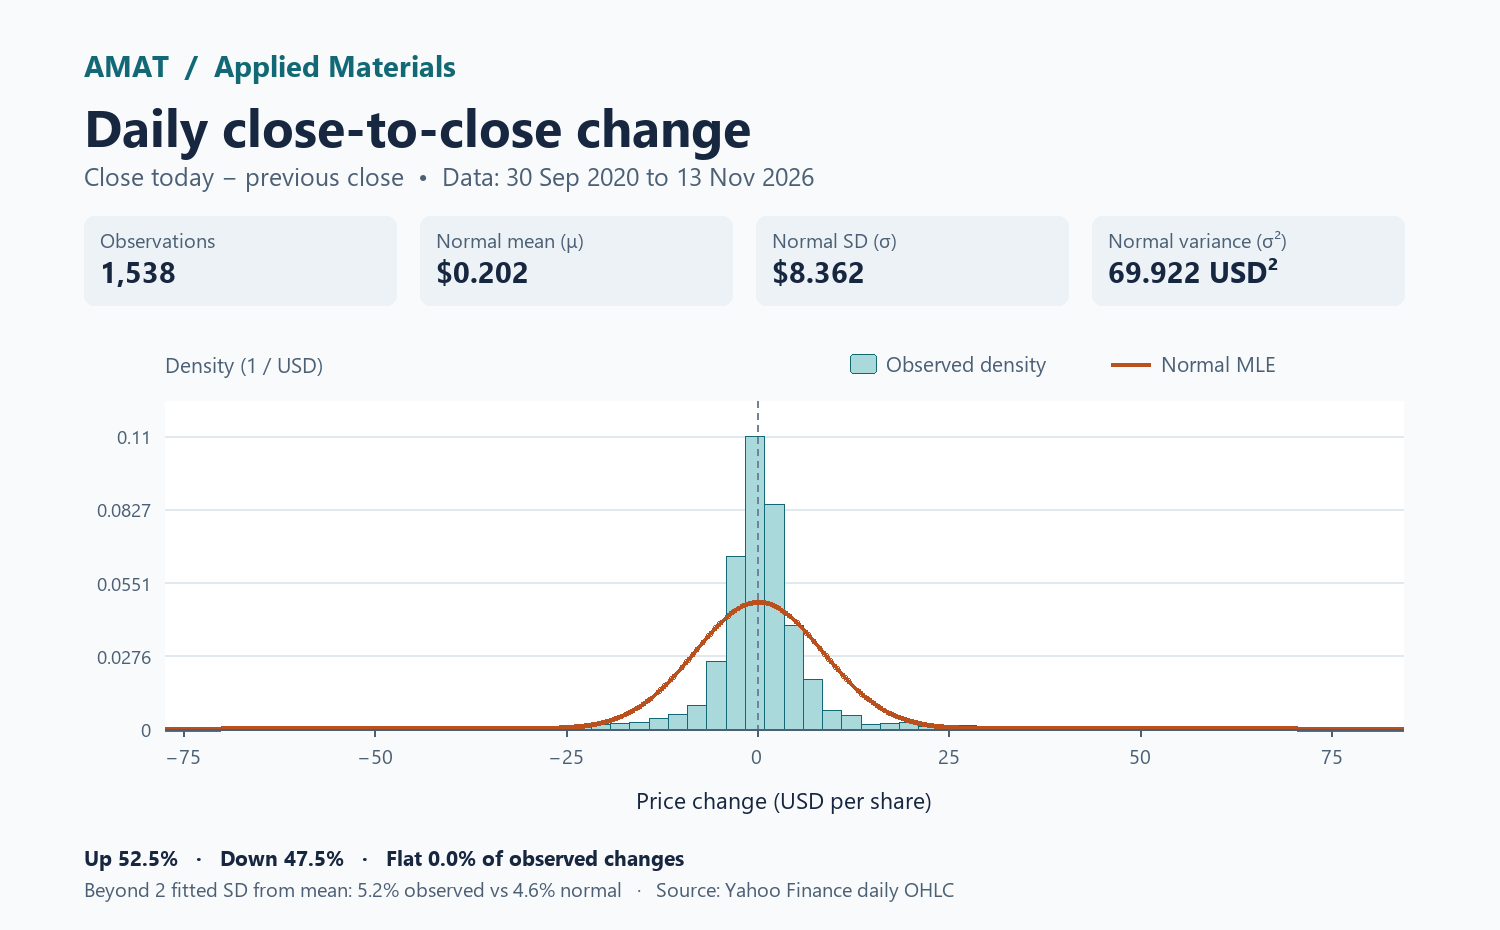
\includegraphics[width=\linewidth,height=2.4cm,keepaspectratio]{ds_normal.png}

{\scriptsize $dS_t$ vs. MLE Normal}
\end{column}
\begin{column}{0.49\textwidth}
\centering
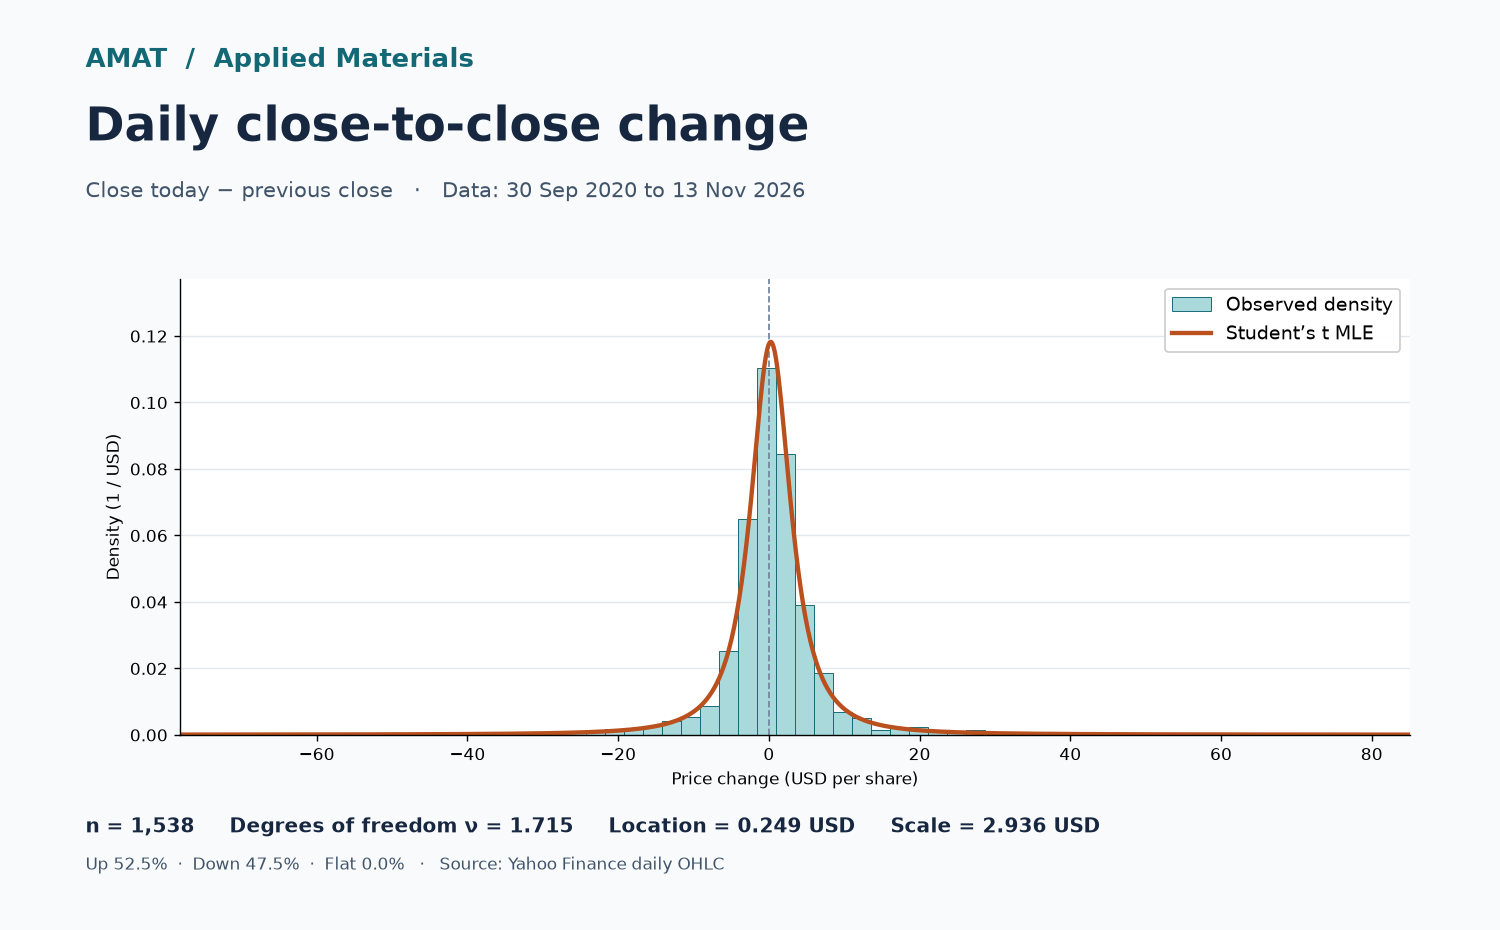
\includegraphics[width=\linewidth,height=2.4cm,keepaspectratio]{ds_student_t.png}

{\scriptsize $dS_t$ vs. MLE Student-t}
\end{column}
\end{columns}
\vspace{0.1cm}
\centering
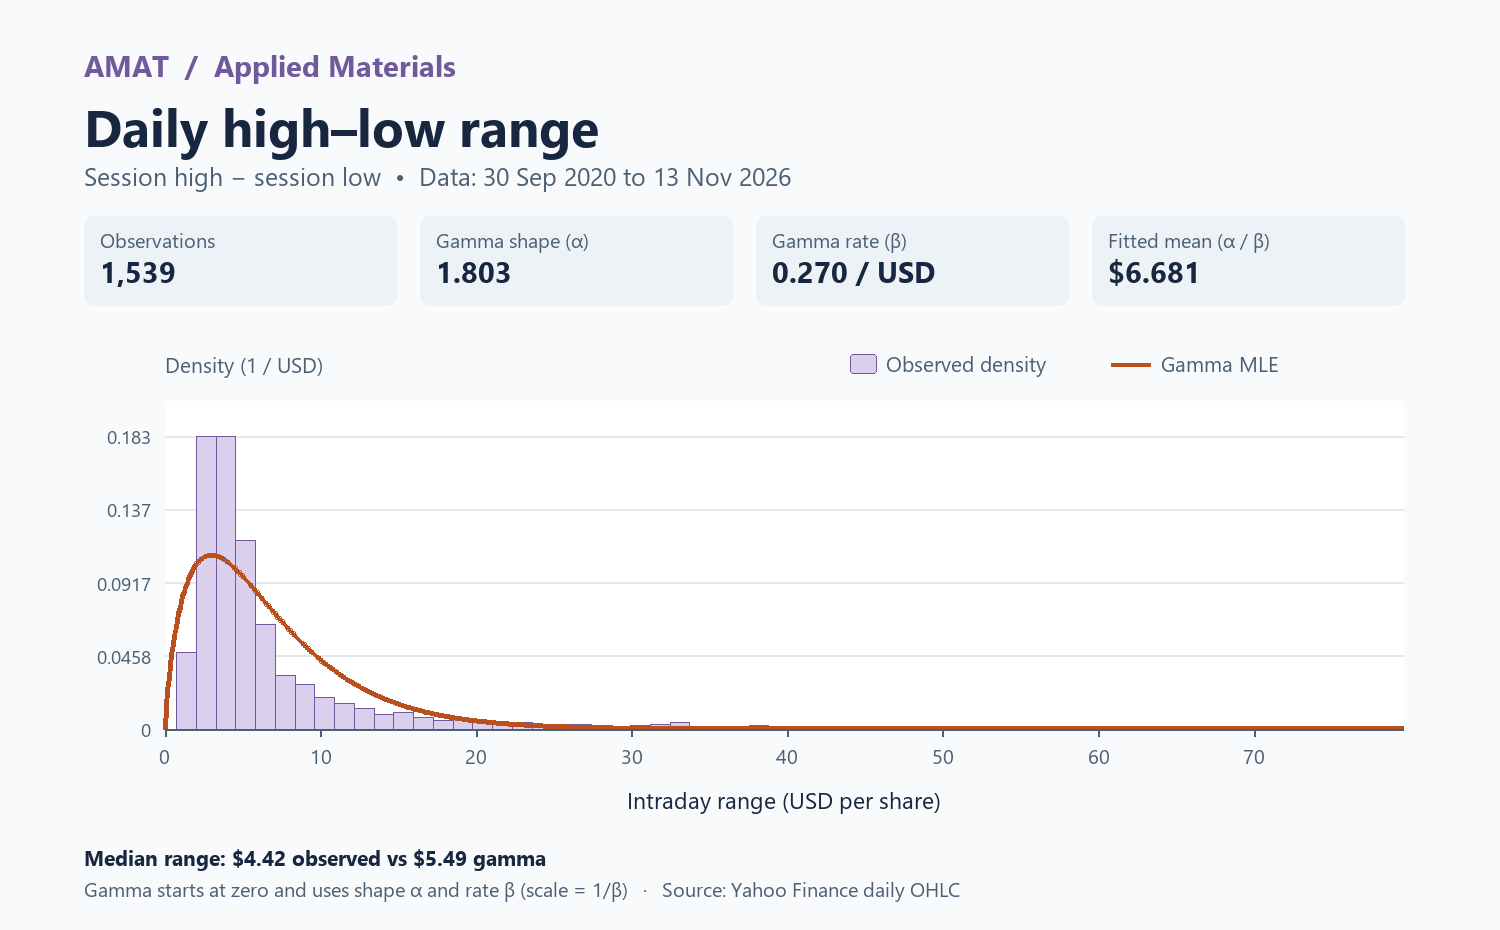
\includegraphics[width=0.55\linewidth,height=2.55cm,keepaspectratio]{hl_gamma.png}

{\scriptsize Intraday Range ($H_t-L_t$) vs. MLE Gamma}
\end{column}
\end{columns}
\end{frame}

\begin{frame}{4. Baseline Modeling: Deterministic Time-Basis Regression}
\small
\begin{columns}[T]
\begin{column}{0.40\textwidth}
\begin{block}{Formulation: $h_\theta(t)=\theta^\top\phi(t)$}
Predicting $S_s$ ($s>t$) conditioned on $\mathcal F_t$ via deterministic basis expansions:
\begin{itemize}
\item \textbf{Polynomial:} $\phi(t)=[1,t,t^2,\dots,t^d]^\top$
\item \textbf{Trigonometric-Poly:} $t^k\cos(t)+t^k\sin(t)$
\item \textbf{Polylogarithmic:} $\operatorname{Li}_s(t)$ basis terms
\end{itemize}
\end{block}
\vspace{0.1cm}
\begin{alertblock}{Critical Questions}
\begin{itemize}
\item \textbf{Why} did all deterministic basis maps yield poor out-of-sample performance?
\item \textbf{Why} is fitting a direct curve $S(t)$ fundamentally ill-posed for equity prices?
\end{itemize}
\end{alertblock}
\end{column}
\begin{column}{0.58\textwidth}
\centering
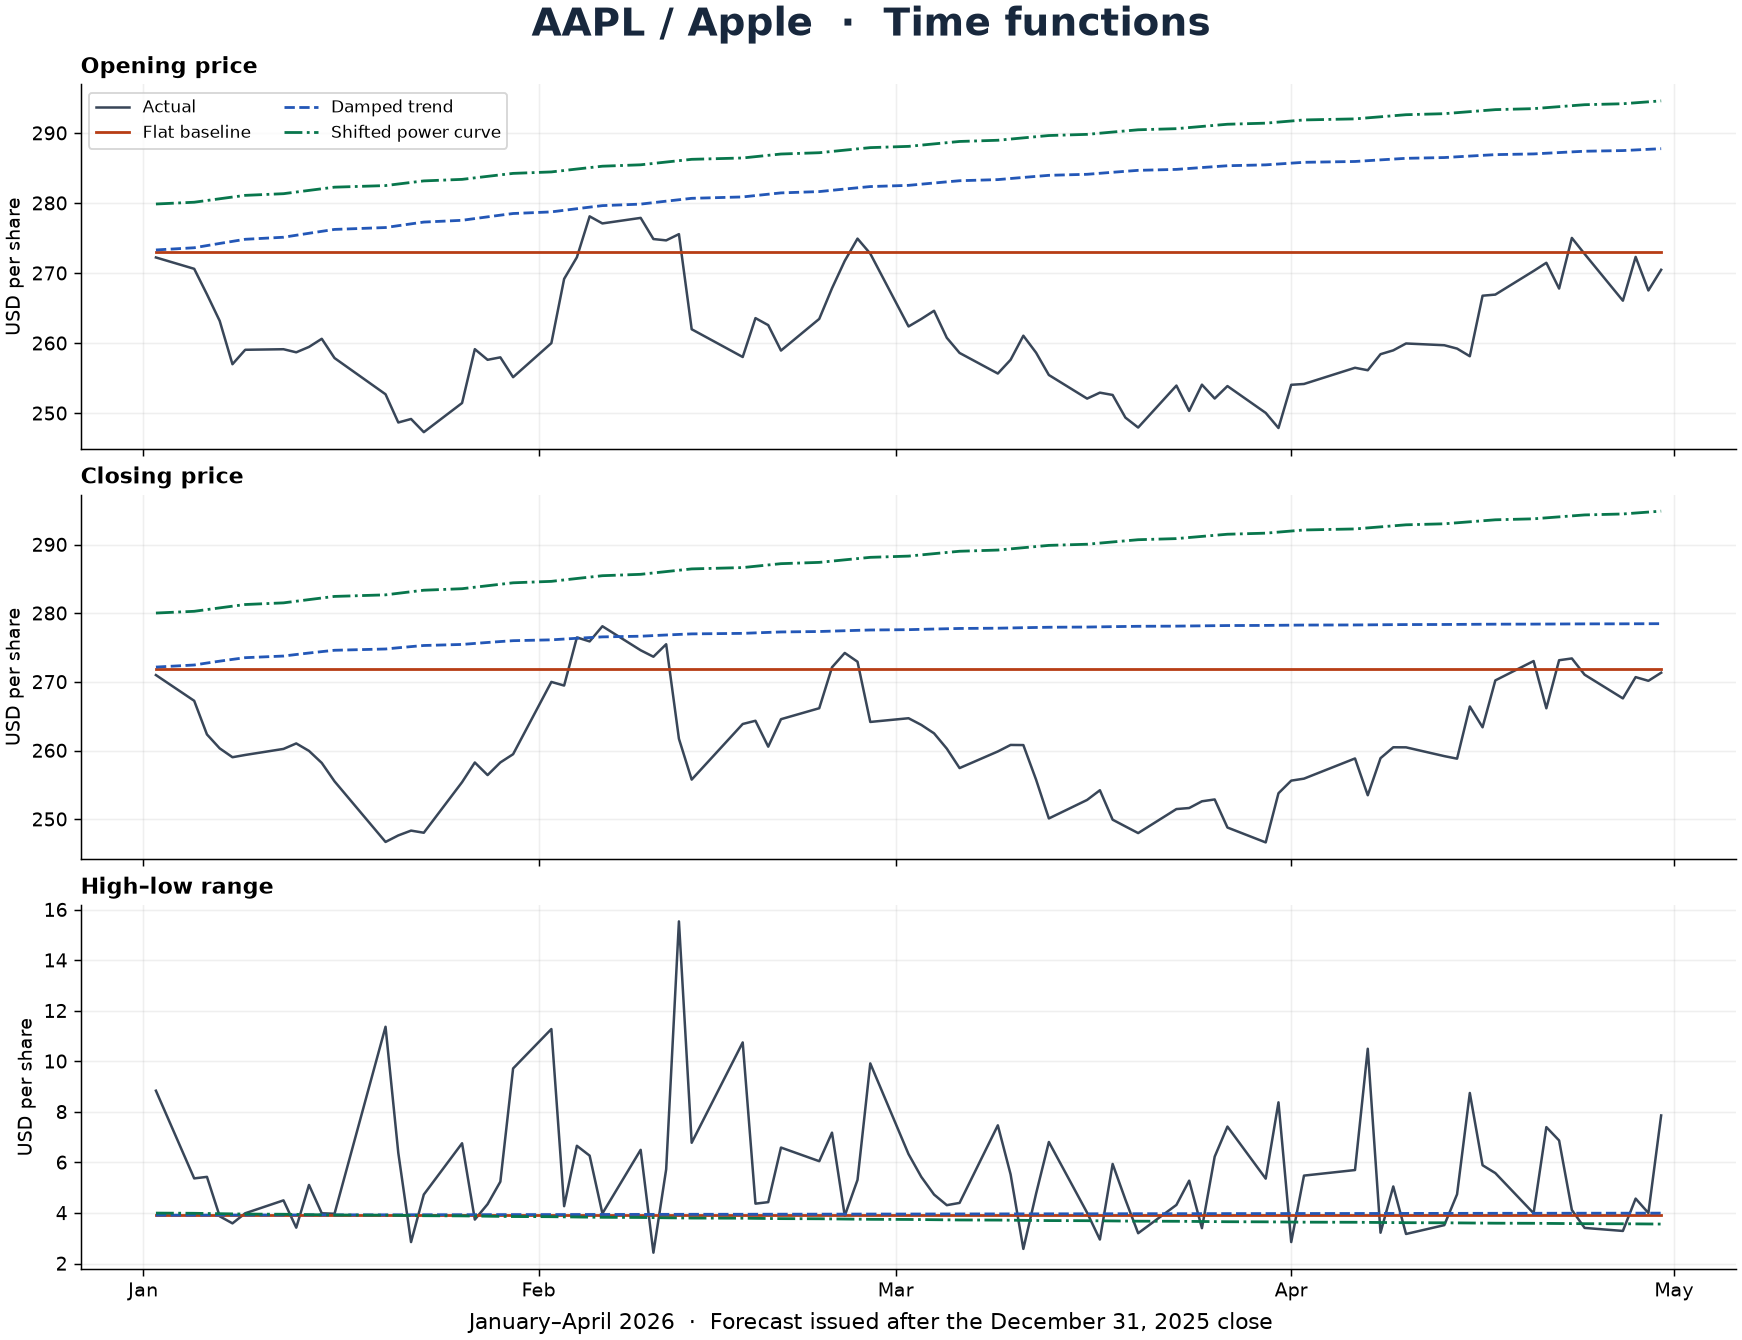
\includegraphics[width=\linewidth,height=2.65cm,keepaspectratio]{AAPL_time.png}

{\scriptsize AAPL Time-Basis Regression vs. Real}

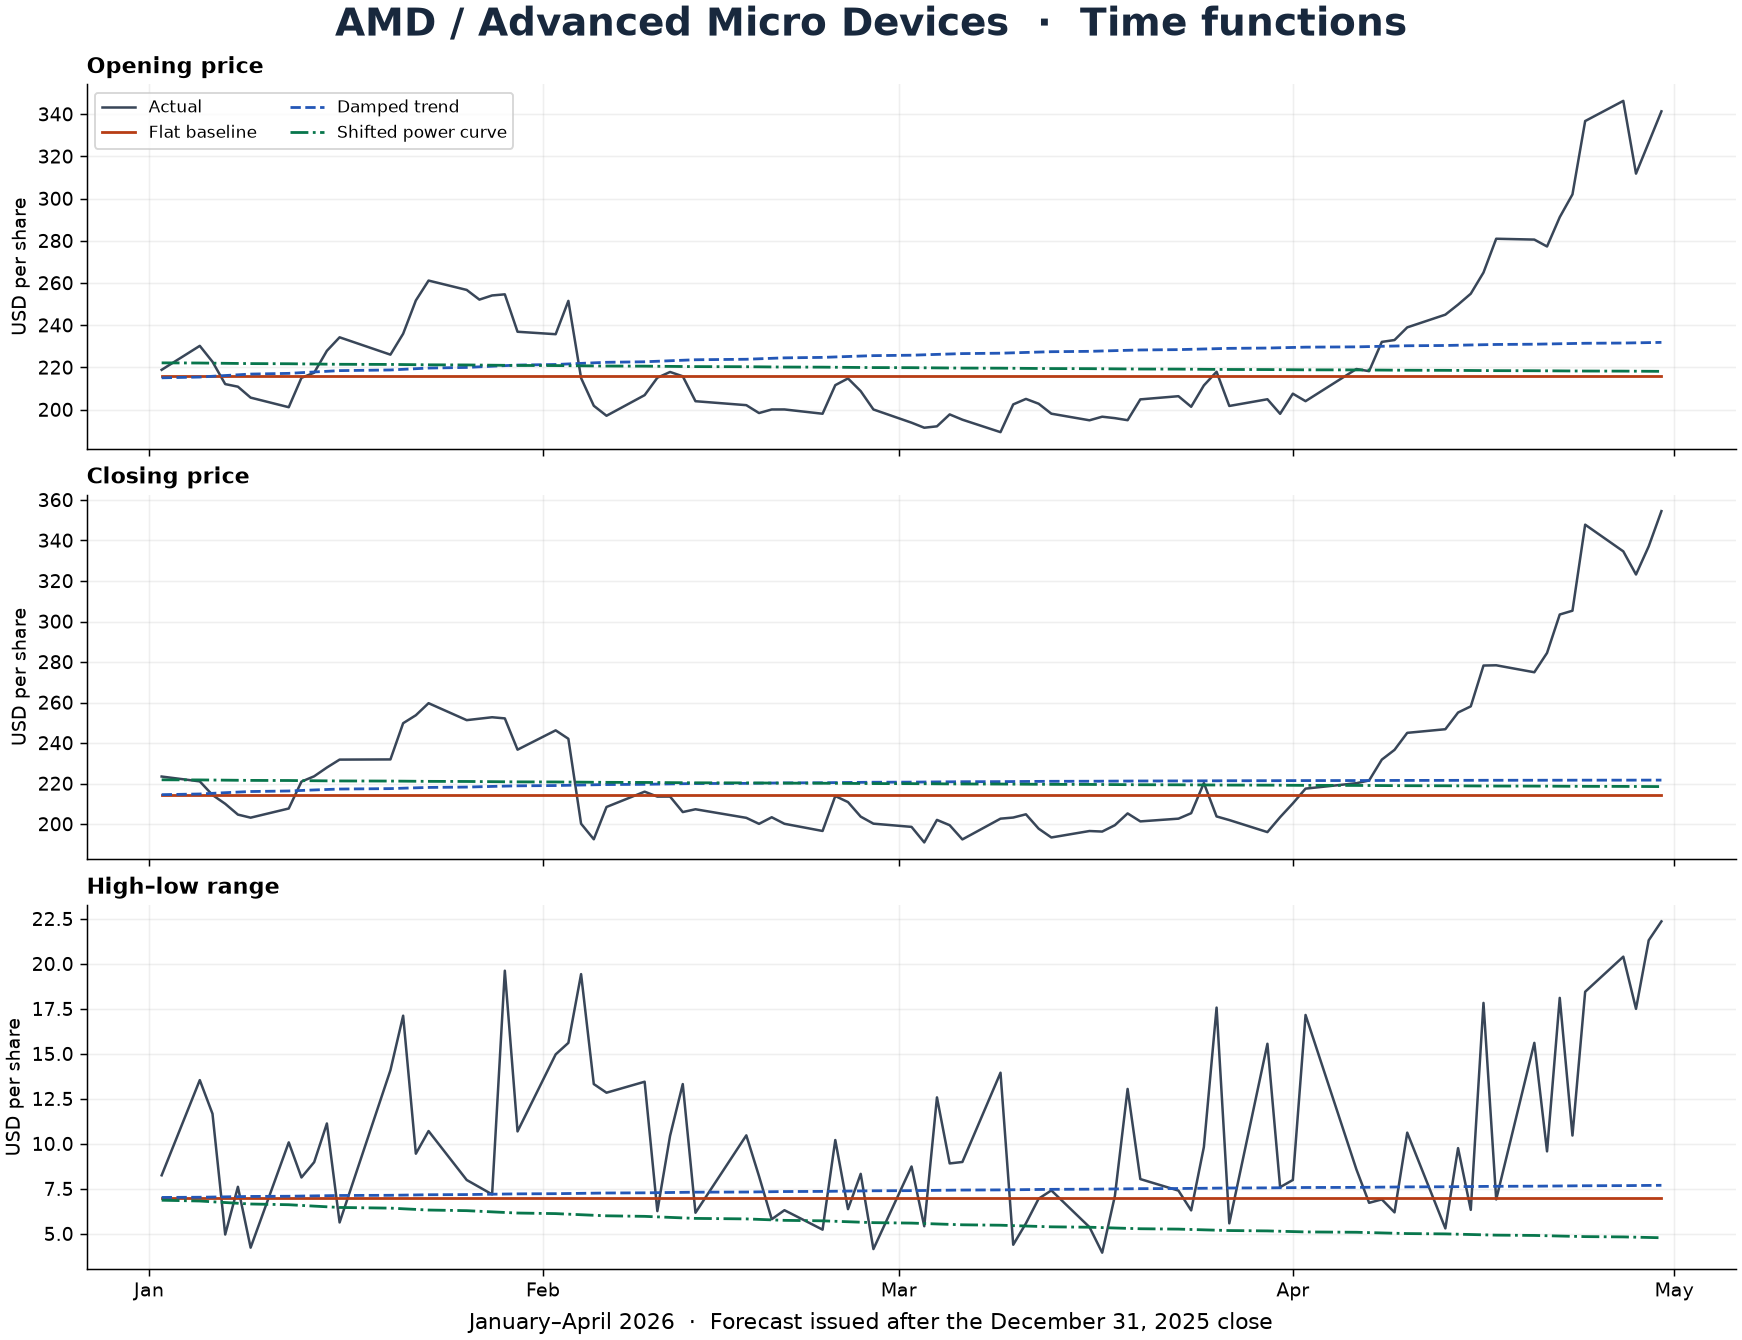
\includegraphics[width=\linewidth,height=2.65cm,keepaspectratio]{AMD_time.png}

{\scriptsize AMD Time-Basis Regression vs. Real}
\end{column}
\end{columns}
\end{frame}

\begin{frame}{5. Autoregressive, Recurrent \& Stochastic Baselines}
\begin{block}{Evaluated Architectures (Strictly Conditioned on $\mathcal F_t$)}
\begin{enumerate}
\item \textbf{Autoregressive Linear (AR-$k$):}
\[
h_\theta(x)=\theta^\top\phi(x),\quad \phi(x)=[S_{t-1},\dots,S_{t-k}]^\top
\]
\item \textbf{Vanilla RNN:} Sequential hidden-state recurrence $h_t=\sigma(W_hh_{t-1}+W_xS_t)$
\item \textbf{LSTM:} Gated memory cells capturing long-range temporal dependencies
\item \textbf{Causal Student-$t$ Random Walk:}
\[
S_{t+1}=S_t+T_t,\quad T_t\sim t(\hat\nu_t,\hat\mu_t,\hat\sigma_t\mid\mathcal F_t)
\]
\end{enumerate}
\centering
{\footnotesize *(MLE parameters estimated strictly on $\mathcal F_t$, eliminating look-ahead bias)*}
\end{block}
\end{frame}

\begin{frame}{6. Empirical Comparison: AR-$k$, RNN, LSTM \& Causal $t$-Walk}
\begin{columns}[T]
\begin{column}{0.49\textwidth}
\centering
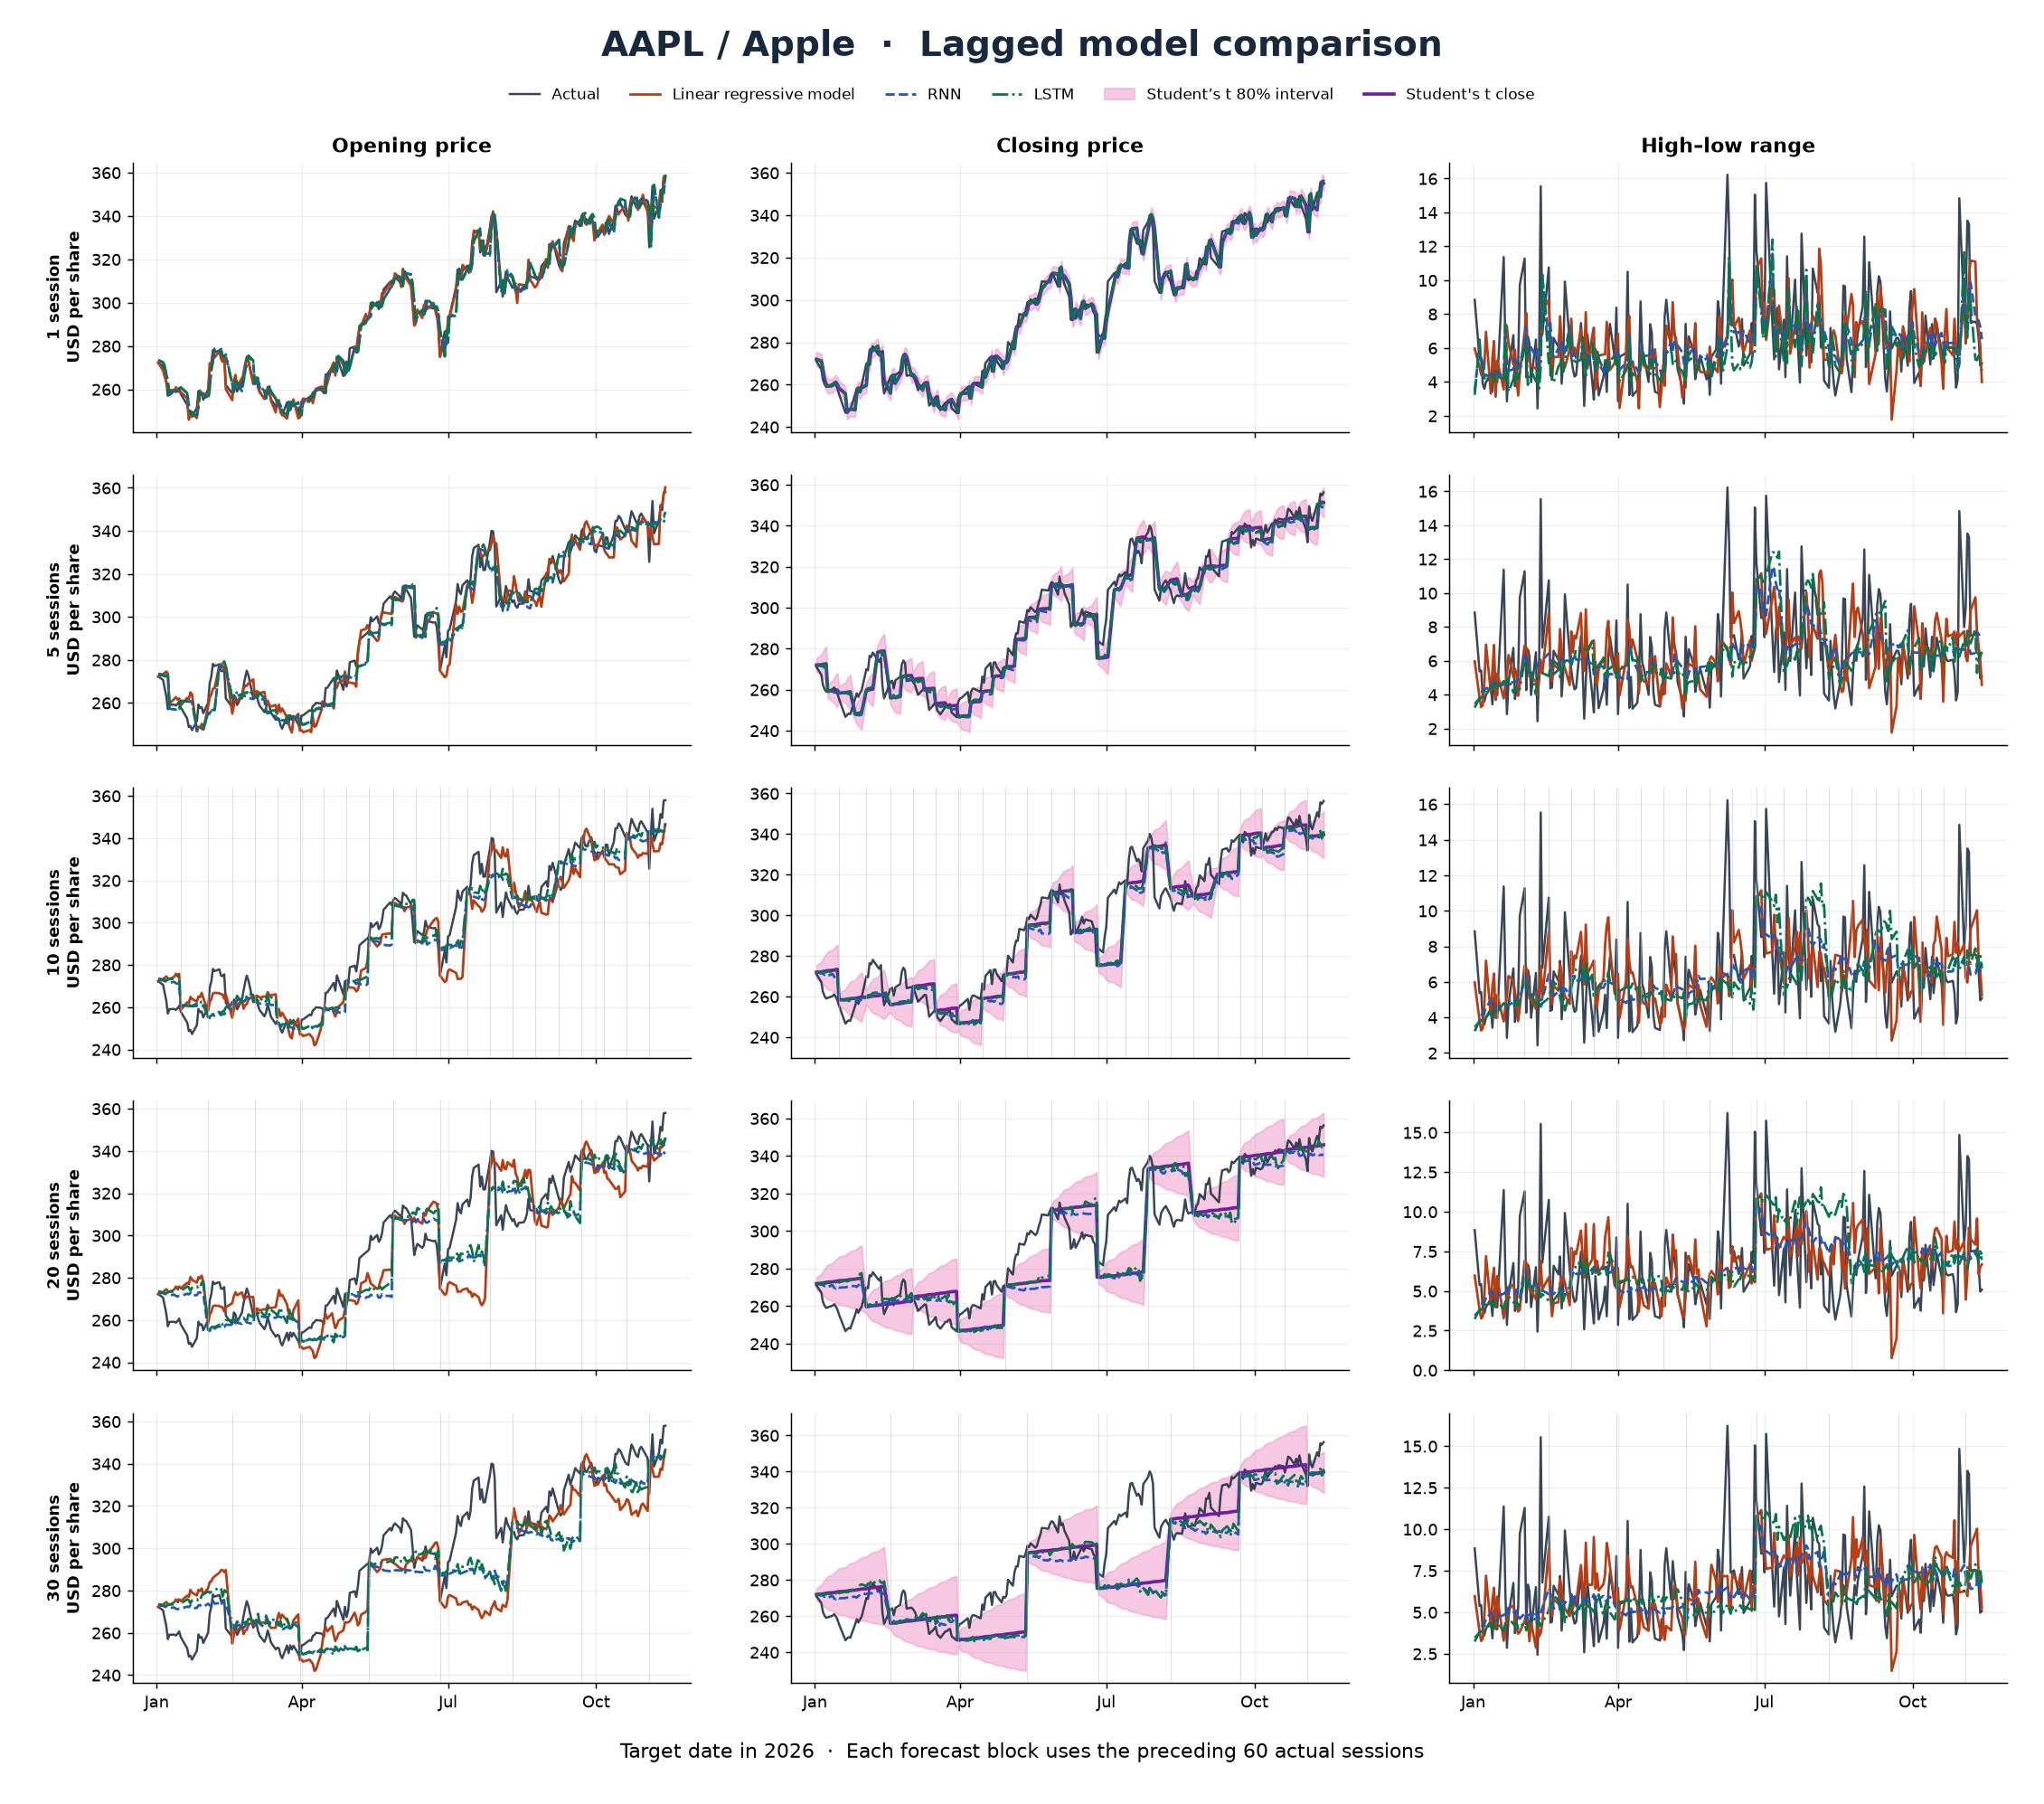
\includegraphics[width=\linewidth,height=5.55cm,keepaspectratio]{AAPL_comparison.png}

{\small \textbf{AAPL:} Out-of-Sample Trajectory Comparison}
\end{column}
\begin{column}{0.49\textwidth}
\centering
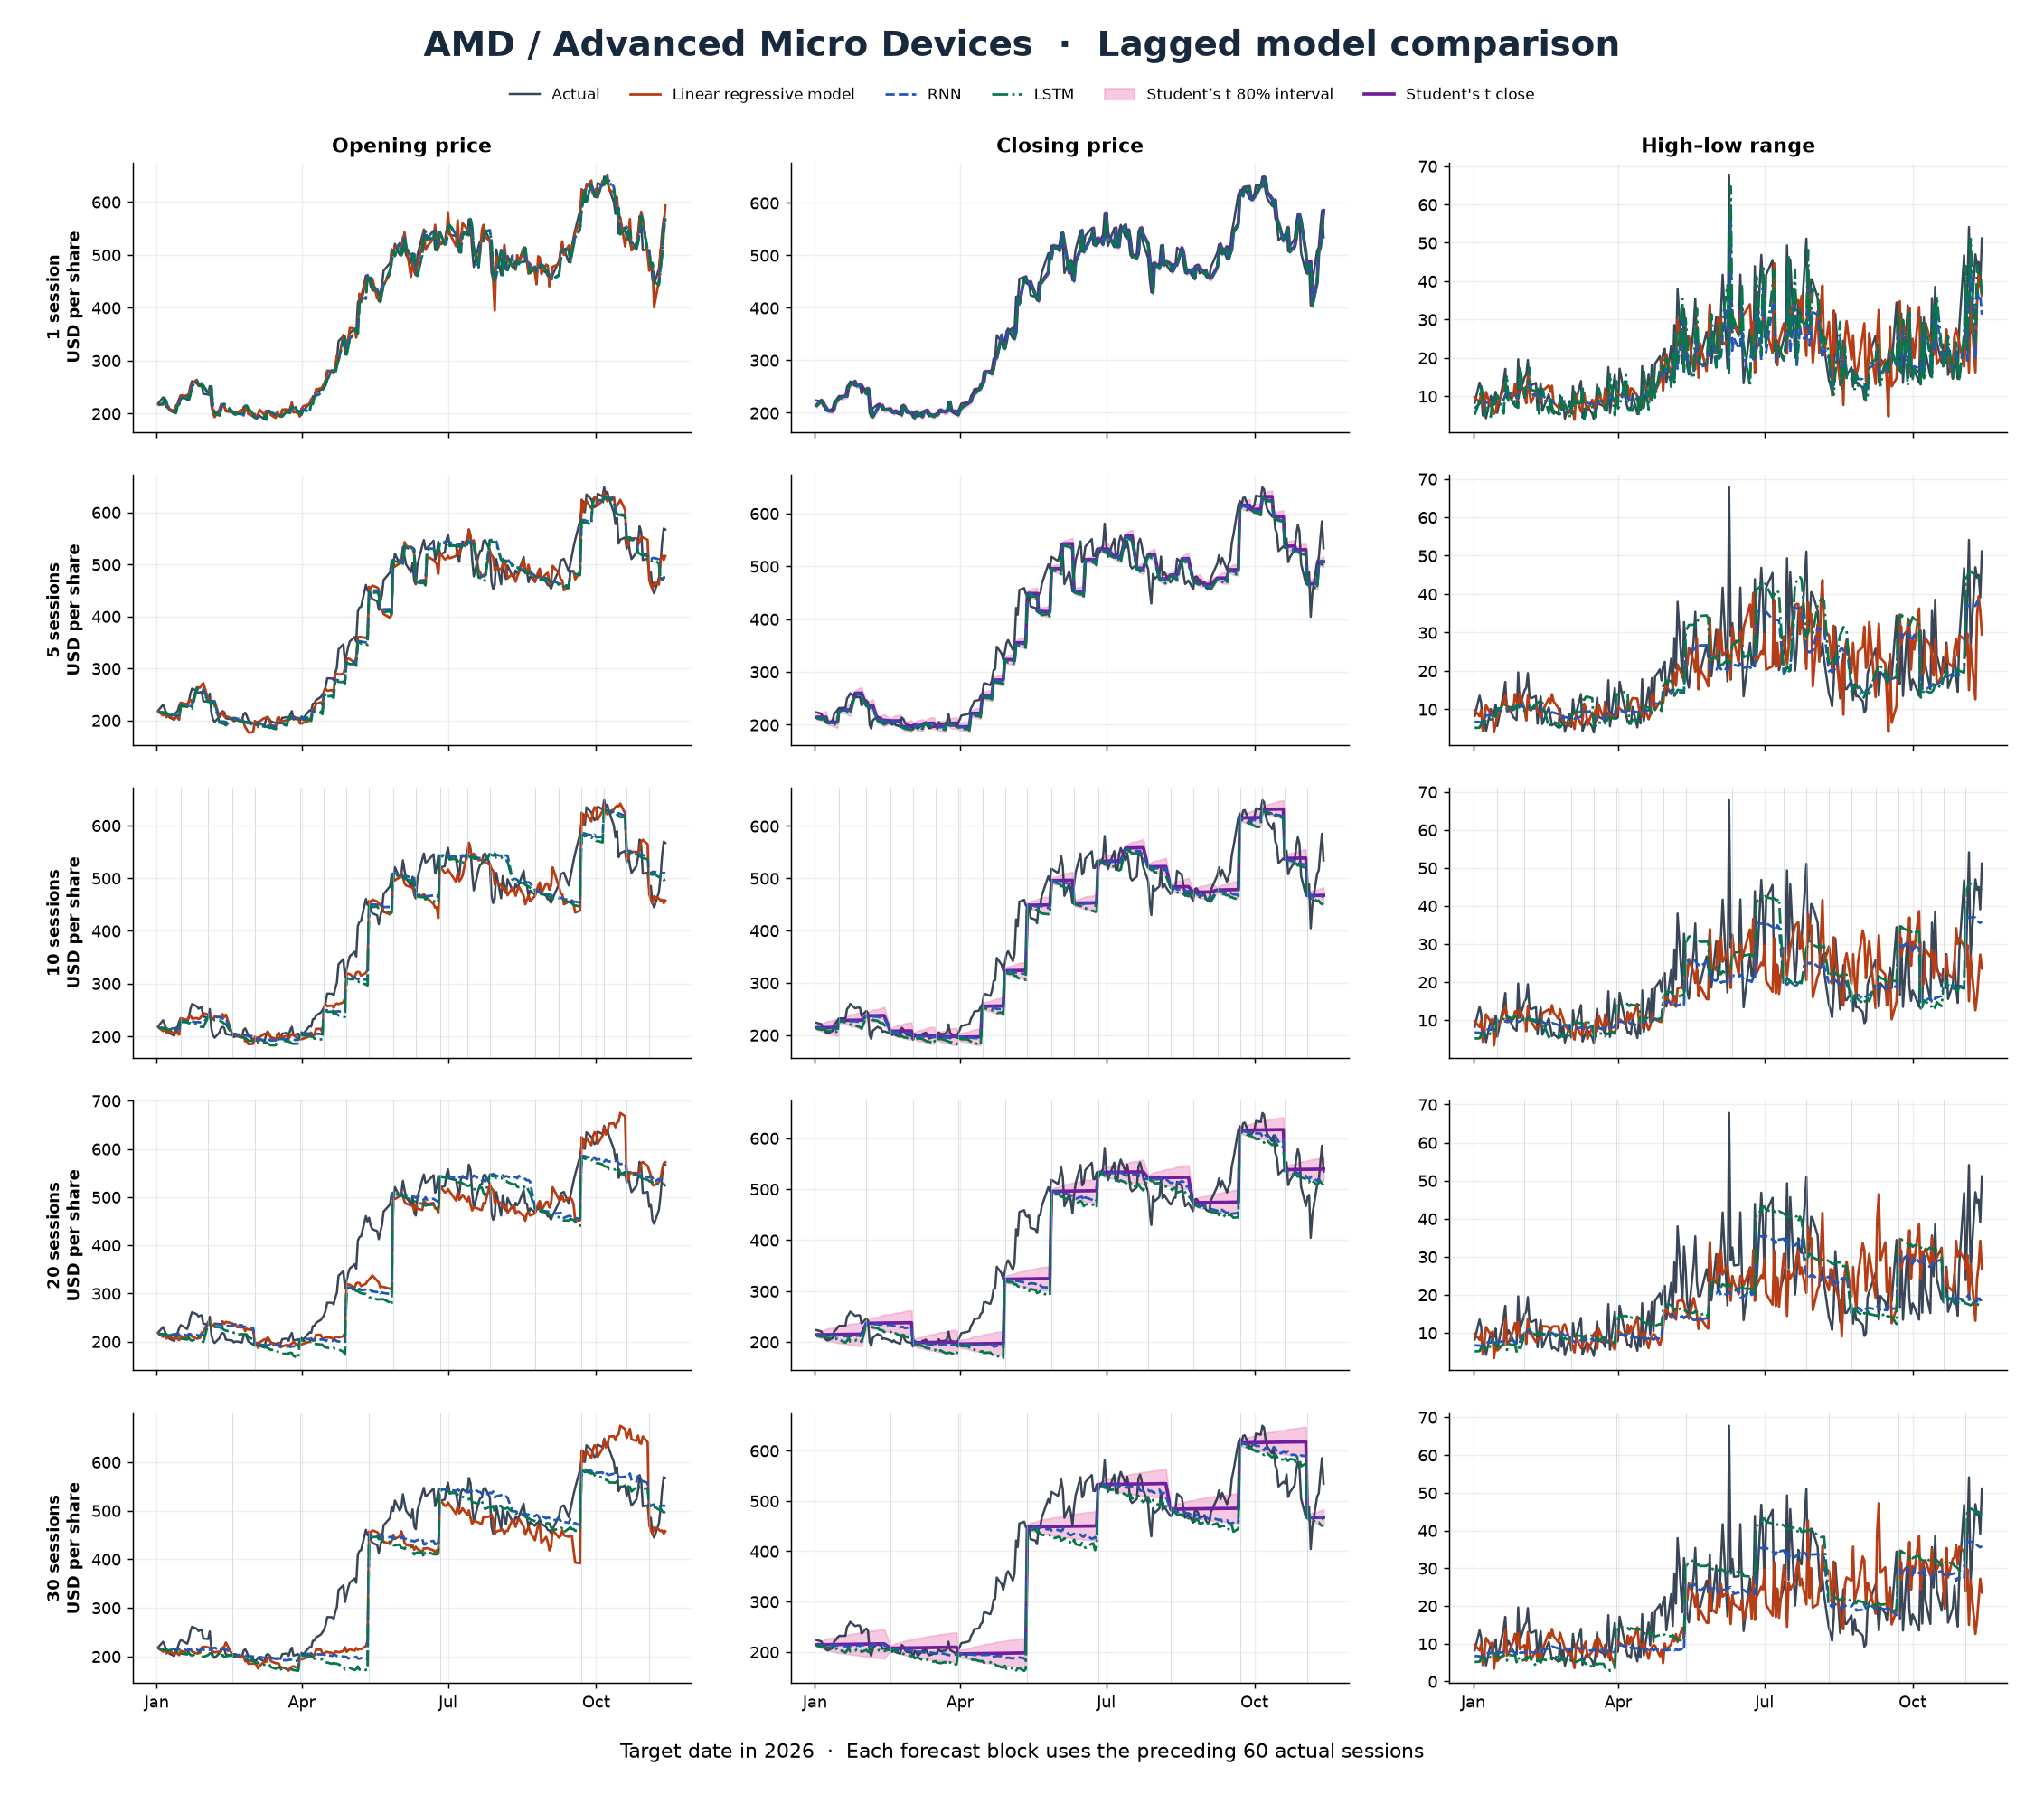
\includegraphics[width=\linewidth,height=5.55cm,keepaspectratio]{AMD_comparison.png}

{\small \textbf{AMD:} Out-of-Sample Trajectory Comparison}
\end{column}
\end{columns}
\end{frame}

\begin{frame}{7. Roadmap: Multi-Horizon Density \& Derivative Pricing}
\begin{columns}[T]
\begin{column}{0.49\textwidth}
\begin{block}{Next-Phase Architectures}
\begin{itemize}
\item \textbf{Rigorous Stochastic Modeling:} State-dependent volatility \& regime-switching dynamics
\item \textbf{Deep Probabilistic Models:} Mixture Density Networks (MDNs), Neural SDEs, Transformers
\item \textbf{Expanded Feature Space:} Integrating $H_t,L_t$ spreads and cross-asset correlations
\end{itemize}
\end{block}
\end{column}
\begin{column}{0.49\textwidth}
\begin{block}{Multi-Horizon Conditional Density ($t<T$)}
\begin{itemize}
\item \textbf{Target Density:} Full transition law for $dS_{t,T}:=S_T-S_t$:
\[
p_t(dS_{t,T}\mid S_t,\mathcal F_t)
\]
\item \textbf{Bayesian Trend Estimator:}
\[
\widehat{dS}_{t,T}=\mathbb E[dS_{t,T}\mid S_t,\mathcal F_t]
\]
\item \textbf{Derivative Pricing:} Deduce forward prices ($F_{t,T}=S_t+\mathbb E^{\mathbb Q}[dS_{t,T}\mid\mathcal F_t]$) \& option payoffs
\item \textbf{Core Challenge:} Empirical sparsity across horizons $(t,T)$ requires parametric/neural density estimation
\end{itemize}
\end{block}
\end{column}
\end{columns}
\end{frame}
\end{document}
